\documentclass[a4paper,14pt,oneside]{extreport}
\usepackage[T2A]{fontenc}
\usepackage[utf8]{inputenc}
\usepackage[english,russian]{babel}
\usepackage{amssymb,amsfonts,amsmath,mathtext,cite,enumerate,float}
\usepackage{indentfirst}
\usepackage[dvips]{graphicx}

\usepackage{fancyvrb,relsize}
\DefineVerbatimEnvironment{VerbatimCode}{Verbatim}%
      {fontsize=\relsize{-2}}

\usepackage{geometry} % Меняем поля страницы
\geometry{left=2cm}% левое поле
\geometry{right=1.5cm}% правое поле
\geometry{top=1.5cm}% верхнее поле
\geometry{bottom=2cm}% нижнее поле

% Меняем везде перечисления на цифра.цифра
\renewcommand{\theenumi}{\arabic{enumi}}
\renewcommand{\labelenumi}{\arabic{enumi}}
\renewcommand{\theenumii}{\arabic{enumii}}
\renewcommand{\labelenumii}{\arabic{enumi}.\arabic{enumii}.}
\renewcommand{\theenumiii}{\arabic{enumiii}}
\renewcommand{\labelenumiii}{\arabic{enumi}.\arabic{enumii}.\arabic{enumiii}.}

\renewcommand{\figurename}{Рис.}
\renewcommand{\bibname}{Использованные источники} % \refname для article и proc!


\title{Электронный каталог книг}
\author{Сафронов М. А.}
\date{Август 2010 г.}

\begin{document}
\begin{titlepage}
\maketitle
\end{titlepage}

\setcounter{page}{2}

\tableofcontents

\newpage

\chapter{Введение}
В данной работе рассматривается разработка электронного каталога книг, основанного на использовании современных веб-технологий: XML/XSLT \\ и Javascript.
Предусмотрен механизм конвертирования исходных данных во внутренний формат каталога при помощи легко доступного интерпретатора Perl.

Цель работы --- создание перечня книг с возможностью поиска и фильтрации по категориям, для просмотра, создания и обслуживания которого требуется как можно меньше специализированного программного обеспечения, в идеале --- только веб-браузер.

При наличии более чем двухсот книг в домашней библиотеке появляется проблема поиска книг и проверки их существования. Наличие удобного электронного каталога, доступного для просмотра непосредственно в веб-браузере, очевидно нивелирует эту проблему, поэтому данная задача представляется актуальной.

Для достижения поставленной цели требуется решить следующие задачи:
\begin{enumerate}
\item реализовать ввод данных в каталог наиболее простым и очевидным способом;
\item реализовать трансформацию исходных данных во внутренний формат каталога;
\item реализовать вывод данных в удобном для просмотра виде;
\item реализовать возможность поиска книг по подстроке в описании и фильтрацию книг по категориям;
\item каталог должен быть доступен для просмотра с использованием как можно меньшего количества специализированного программного обеспечения.
\end{enumerate}

Данный каталог предназначается для хранения сведений об относительно небольшом количестве книг, предположительно до двух тысяч. Им должно быть удобно пользоваться без хардкорной IT-подготовки, для учёта книг в личной домашней библиотеке.

\chapter{Теоретические соображения}

\section{Ввод первоначальных данных}

Специализированные языки разметки и сериализации данных, такие, как JSON и YAML, избыточно сложны для данной задачи, по двум причинам:
\begin{enumerate}
\item присутствуют синтаксические конструкции, пусть и упрощённые, назначение которых требуется специально изучать;
\item требуется использовать повторяющиеся элементы языка, необходимые только для разметки текста: \textit{названия} \textit{пар} в \textit{объектах} для JSON\footnote{См., например, \cite{JSON-spec}} или отступы слева для YAML\footnote{См. \cite{YAML-spec}}.
\end{enumerate} 

Очевидно, исходные данные удобнее всего вводить в неразмеченном виде, друг за другом, построчно, один атом информации о книге на строке. Для компромисса между удобством ввода и удобством обработки было выполнено некоторое сокращение этого представления, и в результате был сформирован следующий формат ввода исходных данных.

\label{rawdata-explained}Все книги описываются в одном текстовом файле. Каждая книга описывается пятью строчками:

\begin{VerbatimCode}
Название книги
Автор книги
Издательство, Город издания, Год издания
Тематическая категория, Краткое описание 
Количество страниц, Физическое состояние книги, Название файла изображения книги
\end{VerbatimCode}

Запятые имеют значение, они играют роль разделителей атомов информации. Таким образом, запятые допускаются только в поле <<Название книги>> и в поле <<Автор книги>>.

Блоки информации о книгах отделяются друг от друга произвольным количеством пустых строчек.

Поле <<Название файла изображения книги>> требуется в том случае, если на момент ввода исходных данных уже имеется изображение книги (фотография в электронном виде). В противном случае его можно пропустить.

\section{Формат хранения данных в каталоге}
В качестве внутреннего формата хранения данных решено использовать XML\footnote{Extensible Markup Language, \cite{XML-spec}}. Для данного языка разметки существует сопутствующий язык XSLT\footnote{Extensible Stylesheet Language for Transformations, \cite{XSLT-spec}}, обработка инструкций на котором поддерживается всеми современными браузерами, и, таким образом, решается одновременно и задача представления данных для пользователя.

\subsection{XML кратко}
Цитата из стандарта XML 1.0, пятая редакция (\cite{XML-spec}), раздел 3, <<Логическая структура>> (перевод автора):

\begin{quote}
Каждый XML документ содержит один или более элементов, границы которых отделены или стартовым и конечным \textit{тегом}, или, для пустых элементов, \textit{тегом} пустого элемента. Каждый элемент имеет тип, обозначенный названием, иногда называемым его <<обобщённым идентификатором>>, и может иметь набор спецификаций атрибутов. Каждая спецификация атрибута имеет имя и значение.\footnote{Definition: Each XML document contains one or more elements, the boundaries of which are either delimited by start-tags and end-tags, or, for empty elements, by an empty-element tag. Each element has a type, identified by name, sometimes called its "generic identifier" (GI), and may have a set of attribute specifications. Each attribute specification has a name and a value}
\end{quote}

Технически XML-документ является текстовым файлом, последовательностью символов, часть которых формирует синтаксические элементы XML и используется для разметки текста. Элемент, содержимое которого обрамлено стартовым и конечным \textit{тегами}, выглядит в XML-документе так:
\begin{VerbatimCode}
<тег-с-названием-элемента>
	<тег-с-названием-вложеннного-элемента>
		Элементы могут содержаться в других элементах,
		образуя древовидную иерархию.
	</тег-с-названием-вложеннного-элемента>
</тег-с-названием-элемента>
\end{VerbatimCode}

Пустой элемент выглядит в XML-документе так:
\begin{VerbatimCode}
<тег-с-названием-пустого-элемента атрибут="значение атрибута" />
\end{VerbatimCode}
Для наглядности в предыдущем примере присутствует демонстрация присваивания \textit{тегам} \textit{атрибутов}.

XML-документ должен содержать один и только один \textit{корневой элемент}, который содержит в себе все остальные элементы документа.
	
\section{Преобразование исходных данных}
Для преобразования исходных данных в XML-формат, используемый каталогом, решено было использовать возможности языка Perl.\footnote{Для языка отсутствует формальная спецификация. Официальный веб-узел: \cite{Perl-website}, документация: \cite{Perl-docs}} Perl является интерпретируемым языком программирования, изначально разработанным для удобства обработки массивов текста. Интерпретатор Perl доступен для всех основных сочетаний аппаратных и программных платформ. Для Windows есть сборка интерпретатора Perl от фирмы ActiveState, под названием ActivePerl, см.~\cite{ASPerl-website}, она учитывает особенности как самой операционной системы, так и основной её аудитории. 

Следующие две причины послужили поводом для выбора Perl в качестве языка разработки:
\begin{itemize}
\item интерпретируемый язык позволяет наиболее простым способом изучать и менять поведение программы --- прямым редактированием её исходного текста;
\item изначальный дизайн языка Perl предполагает использование его для написания программ обработки текстов, он включает в себя удобные языковые конструкции для этого.
\end{itemize}

Синтаксис Perl в целом похож на гораздо более широко известный C/C++. Описание языка здесь излишне, в качестве справочного пособия можно порекомендовать книгу издательства O'Reilly под названием Programming Perl (\cite{Perl-o-reilly-book}), в сообществе пользователей Perl она считается нормативной.

В дальнейшем условимся, вследствие интерпретируемости языка Perl, называть программы, написанные на этом языке, \textit{скриптами}.

Предполагается, что framework каталога будет включать в себя скрипт для трансформации исходных данных о книгах в XML-формат, годный для использования в каталоге. Он должен вызываться наиболее простым возможным способом, например, вызовом в командной строке операционной системы команды:
\begin{VerbatimCode}
perl books-to-catalog.pl
\end{VerbatimCode}

Здесь \verb'perl' --- это команда вызова интерпретатора Perl, \verb'books-to-catalog.pl' --- название скрипта трансформации. Название исходного файла и название файла конечного XML-документа скрипт должен предположить самостоятельно, либо они должны быть оговорены заранее.

\section{Отображение каталога}
Для отображения каталога из XML-формата решено использовать язык XSLT \cite{XSLT-spec}.

XSLT --- это язык разметки, который позволяет описать преобразование исходного XML-документа в любой другой произвольный формат\footnote{\cite{XSLT-spec} однозначно утверждает, что XSLT предназначен для преобразования XML-документов в XML-документы, однако одновременно с этим определяет метод вывода в виде обычного текста, откуда ясно, что формат результата может быть любым}. XSLT является производным от XML, поэтому документы на этих языках имеют одинаковую логическую структуру --- иерархическое дерево вложенных друг в друга элементов, обозначенных \textit{тегами}.

В данном проекте XSLT будет использован для того, чтобы преобразовать XML-документ, хранящий каталог книг, в XHTML-документ\footnote{XHTML \cite{XHTML-spec} является переработкой языка разметки гипертекста HTML \cite{HTML-spec} для соответствия его синтаксису XML. Назначение обоих языков одинаковое.}. Полученный \\ XHTML-документ может быть просмотрен любым веб-браузером, конформным современным веб-стандартам.

Преимущество данного подхода в том, что все ключевые современные веб-браузеры\footnote{Microsoft Internet Explorer, Opera, Mozilla Firefox, Google Chrome и Apple Safari. Везде в дальнейшем именно эти пять веб-браузеров будут называться <<ключевыми современными веб-браузерами>>.} включают в себя поддержку обработки XSLT-документов без использования какого-либо дополнительного программного обеспечения.

\subsection{XSLT кратко}
Рассмотрим XSLT предельно сжато. Подробное описание можно прочитать в спецификации (\cite{XSLT-spec}) или в книге издательства O'Reilly под названием <<XSLT, 2nd Edition>> (\cite{XSLT-o-reilly-book}).

XSLT-документ, описывающий преобразование, называется \textit{stylesheet}\footnote{Традиционный перевод <<таблица стилей>>. Следует учитывать, что <<таблица>> употребляется в смысле <<сводка>>, <<перечень>>, никакой табличной структуры XSLT-\textit{stylesheet} не обладает.}. В \cite{XSLT-spec}, спецификации XSLT, о структуре XSLT-документа сказано следующее (перевод и выделение курсивом автора).
\begin{quote}
Stylesheet состоит из набора \textit{шаблонных правил}. \textit{Шаблонное правило} состоит из двух частей: шаблона, который сравнивается с узлами в исходном дереве и шаблона, экземпляр которого может участвовать в формировании результирующего дерева.\footnote{A stylesheet contains a set of template rules. A template rule has two parts: a pattern which is matched against nodes in the source tree and a template which can be instantiated to form part of the result tree.}
\end{quote}

\textit{Шаблонное правило} выглядит следующим образом:

\begin{VerbatimCode}
<xsl:template match="путь-к-элементу">
	Содержимое, которое будет выведено 
	в результирующее дерево вместо элемента,
	найденного в результате разбора
	значения атрибута match. Может содержать любой текст.
</xsl:template>
\end{VerbatimCode}

Атрибут \verb'match' содержит правило выбора элементов из исходного дерева. Фактически это должно быть валидное выражение на языке XPath\footnote{Язык описания местонахождения в XML-документе. См.~\cite{XPath-spec}}. В простейшем случае значение атрибута match --- название элемента в исходном дереве.

Все элементы, которые будут найдены в результате разбора аргумента \verb'match', будут заменены в результирующем дереве на содержимое текущего элемента \verb'xsl:template'. Этим можно пользоваться, например, для преобразования некоторых элементов исходного XML-документа в элементы HTML, которые будут тем или иным образом отрендерены веб-браузером.

\subsection{Интерфейс каталога}
В простейшем случае XSLT stylesheet, согласно \cite{XML-style-spec}, может быть связан с исходным XML-документом при помощи следующей инструкции обработки:
\begin{VerbatimCode}
<?xml-stylesheet type="text/xsl" href="XSLT-URI" ?>
\end{VerbatimCode}

Благодаря встроенной поддержке обработки XSLT в современных веб-браузерах пользователь может непосредственно открыть этот XML-документ в веб-браузере и получить его преобразованное представление (в простейшем случае --- в XHTML-формате). Однако, для достижения поставленной цели требуется решить задачу реализации фильтрации каталога по категориям а также поиска книг. Фильтрация каталога может быть реализована использованием возможности передавать XSLT-процессору именованные параметры, и учитывать наличие этих параметров в stylesheet'е. Таким образом, требуется иметь программный интерфейс к XSLT-процессору веб-браузера, позволяющий реагировать на команды пользователя и запускать преобразование с заданными определёнными параметрами.

Все ключевые современные веб-браузеры имеют в качестве программного интерфейса язык javascript\footnote{Основан на стандарте ECMAScript, см.~\cite{ECMAScript-spec}. Здесь не будут рассматриваться основы этого весьма распространённого и известного языка программирования}. MS Internet Explorer реализует интерпретатор другого языка, под названием JScript, почти полностью совместимого с javascript. Для доступа к XSLT-процессору в браузерах, отличающихся от Internet Explorer, принят API \cite{Mozilla-JS-XSLT-API}, изначально предложенный компанией Mozilla для использования в своём веб-браузере Firefox. Этот подход основан на манипуляции специальным объектом \verb'XSLTProcessor', прозрачной для javascript. 

В Internet Explorer используется подход, основанный на ActiveX объектах, что является препятствием для кроссбраузерности данного проекта. Одновременно с этим веб-браузеры, отличающиеся от Firefox, реализуют функциональность \verb'XSLTProcessor' с индивидуальными особенностями. Для преодоления данных трудностей в программном интерфейсе разрабатываемого каталога будет использоваться библиотека API для javascript под названием Sarissa (см. ~\cite{Sarissa-website}). Использование Sarissa позволяет в программном коде использовать подход Mozilla для доступа к XSLT процессору браузера и данный код будет выполняться в любом ключевом современном браузере единообразно\footnote{По крайней мере, в идеальном случае. Как будет показано ниже, веб-браузеры, основанные на движке Webkit, Chrome и Safari в версиях, актуальных на август 2010, всё равно интерпретируют код вывода каталога некорректно.}

Для удобства разработки программной части каталога решено использовать библиотеку для javascript под названием jQuery (см.~\cite{jQuery-website}), и её ответвление, инкапсулирующее некоторые дополнительные элементы интерфейса, под названием jQueryUI (jQuery User Interface, см.~\cite{jQueryUI-website}).

Таким образом, абстрактно схема работы каталога будет следующей.
\begin{enumerate}
\item Пользователем в веб-браузере открывается стартовая страница каталога. Это XHTML-документ.
\item Веб-браузер при рендеринге стартовой страницы подгружает необходимые для работы программные интерфейсы: Sarissa, jQuery, jQueryUI.
\item Запускается код javascript, инициирующий формирование интерфейса каталога --- в первом приближении фильтра по категориям и кнопки запуска отбора книг из каталога.
\item Пользователь запускает отбор книг из каталога. Формируется вызов XSLT процессора, который трансформирует исходный XML-документ со сведениями о книгах в таблицу с результирующими данными.
\item Полученные от XSLT процессора данные выводятся на веб-страницу каталога, открытую в браузере.
\end{enumerate}

\subsection{Вывод данных}
Сведения, отобранные из XML-документа каталога, выводятся на веб-страницу в виде таблицы.

В одной из колонок отображается уменьшенная копия изображения книги, по нажатию на которую открывается полноразмерное изображение книги. Для реализации этого требуется предусмотреть хранение как полноразмерных изображений, так и их уменьшенных копий.

Существует дополнительный плагин для jQuery, под названием DataTables (см.~\cite{jQuery-DataTables}), который предназначен для автоматизированного преобразования указанной таблицы в HTML-документе. DataTables дополняет таблицу простым делением на страницы с регулируемым количеством записей на каждой странице, возможностью пересортировки записей по произвольной колонке и поиском записей по подстроке в любом её поле. Таким образом, на втором шаге потребуется подключить этот плагин, и после вывода таблицы на веб-страницу <<усилить>> её.

\chapter{Детали реализации}
\section{Импорт данных}
Процесс импорта данных представляется следующим.
\begin{enumerate}
\item Данные о книгах заносятся в текстовый документ в виде, описанном в \ref{rawdata-explained}. Имя файла с этим текстовым документом заранее оговорено, в данной работе используется имя \verb'books-data.txt'.
\item В отдельном текстовом документе указывается, каким книгам какой файл изображения соответствует.
\item Запуском скрипта трансформации исходных данных в XML-формат генерируется файл с оговорённым названием (в данной работе используется имя \verb'books-data.xml'), содержащий XML-документ каталога книг.
\item В заранее оговорённом подкаталоге размещаются файлы полноразмерных изображений книг, и в другом заранее оговорённом каталоге --- файлы с thumbnail'ами этих изображений. В данной работе используются подкаталоги \verb'data/images/' и \verb'data/thumbnails' соответственно.
\item Запуском отдельного скрипта на основании текстового документа, упомянутого в пункте 2), в XML-документ каталога внедряются сведения о названиях изображений книг.
\end{enumerate}

Включение в XML-документ каталога названий изображений вынесено в отдельный шаг импорта, потому что это предоставляет возможность ввести данные в каталог, не имея изображений книг либо ввести данные о изображениях в уже существующий каталог.

\subsection{Скрипт импорта данных о книгах}
По умолчанию называется \verb'books-to-xml.pl'. Ожидает входной файл в подкаталоге \verb'data' относительно себя, соответственно под названием \\ \verb'data/books-data.txt'. Генерирует выходной файл \verb'data/books-data.xml'.

\subsection{Скрипт импорта данных об изображениях книг}
По умолчанию называется \verb'books-images-insert.pl'. Ожидает наличие подкаталогов \verb'data/images/' и \verb'data/thumbnails/'. Ожидает входной файл с указаниями под названием \verb'orders.txt'. 

Файл с указаниями содержит набор строчек следующего вида:
\begin{VerbatimCode}
старое название;новое название;книга
\end{VerbatimCode}

Здесь <<старое название>> и <<новое название>> соответственно --- старое и новое названия изображений книги без расширения. По умолчанию расширение считается равным \verb'.jpg'. <<книга>> --- регулярное выражение\footnote{См., например, \cite{regexp-book}}, соответствующее какой-либо из строк описания книги в XML-документе каталога. Это позволяет достаточно изощрённым образом добавлять сведения об изображениях в каталог, однако, является также вынужденно неудобным способом делать это.

Скрипт открывает XML-документ каталога, ожидая его по умолчанию в файле \verb'data/books-data.xml', ищет в нём строку, соответствующую какому-нибудь из регулярных выражений <<книга>>, имеющихся в файле указаний, и, найдя, добавляет в XML-документ строчку, описывающую элемент, содержащий название файла изображения книги. Затем скрипт находит в каталоге \verb'data/images/' файл под названием <<старое название>> и переименовывает его в <<новое название>>. Затем находит в каталоге \verb'data/thumbnails/' файл под названием <<thumb-<<старое название>> и переименовывает его в <<thumb-<<новое название>>.

В исходном коде имеются два флага. Один называется UTF8FS, и он определяет, следует ли при переименовании файлов задавать имя в кодировке cp1251 (требуется для корректной работы в файловой системе FAT, по умолчанию отключено) либо кодировать по современным best practices в UTF-8. Второй называется NOTRANSLIT, и определяет, следует ли переименовывать кириллицу в названиях файлов в транслит или нет (полностью убирает проблему не-ASCII символов в названиях файлов, по умолчанию скрипт переименовывает в транслит).

\section{XML-документ каталога}
Внутренний формат каталога имеет следующий вид:
\begin{VerbatimCode}
<books>
  <book category="Тематическая категория">
    <name>Название</name>
    <image>Файл изображения</image>
    <author>Автор(ы)</author>
    <publisher>Издательство</publisher>
    <city>Город издания</city>
    <year>Год издания</year>
    <description>Краткое описание</description>
    <pagenum>Количество страниц</pagenum>
    <condition>Описание состояния книги</condition>
  </book>
... ещё элементы book ...
</books>
\end{VerbatimCode}

\section{XSLT-документ}
Полный текст см. в файле \verb'books-table-partial.xsl'.

Используется три параметра.
\begin{itemize}
\item \verb'$selector-mode' определяет режим отбора книг;
\item \verb'$category' содержит название категории, по которой следует производить отбор книг;
\item \verb'$show-images' определяет, следует ли выводить колонку с уменьшенными копиями изображений книг (это полезно, если количество изображений слишком велико и вывод данных из-за этого замедляется).
\end{itemize}

Исходный XML-документ каталога трансформируется в набор элементов XHTML, описывающих таблицу. 
\begin{VerbatimCode}
<xsl:template match="/">
  <table id='catalog'>
    <caption>Книги на избавление: <xsl:value-of select="$category" />. 
	Selector mode: <xsl:value-of select="$selector-mode" />
    </caption>
    <thead>
      <tr>
        <xsl:if test="$selector-mode='all'">
          <th>Категория</th>
        </xsl:if>
        <xsl:if test="$show-images">
          <th>Изображение</th>
        </xsl:if>
        <th>Название</th>
        <th>Автор</th>
        <th>Издательство</th>
        <th>Город</th>
        <th>Год</th>
        <th>Описание</th>
        <th>Количество страниц</th>
        <th>Состояние</th>
      </tr>
    </thead>
    <tbody>
  <xsl:choose>
    <xsl:when test='$selector-mode="all"'>
      <xsl:apply-templates select="books/book" />
    </xsl:when>
    <xsl:when test='$selector-mode="category"'>
      <xsl:apply-templates select="books/book[@category=$category]" />
    </xsl:when>
    <xsl:when test='$selector-mode="undef"'>
      <xsl:apply-templates select="books/book[not(@category)]" />
    </xsl:when>
  </xsl:choose>
    </tbody>
  </table>
</xsl:template>
\end{VerbatimCode}

Благодаря использованию параметра \verb'$selector-mode' осуществляется отбор книг из каталога. Реализованы три режима отбора:
\begin{enumerate}
\item все книги;
\item книги, принадлежащие определённой категории;
\item книги, не принадлежащие никакой категории (у элемента \verb'book' отсутствует атрибут \verb'category').
\end{enumerate}

Каждый элемент \verb'book' каталога выводится в виде строки этой таблицы. Каждая колонка этой таблицы соответствует одному из элементов, содержащих сведения о той или иной характеристике книги.
\begin{VerbatimCode}
  <xsl:template match="book">
    <tr>
    <xsl:if test='$selector-mode="all"'>
      <td class="category"><xsl:apply-templates select="@category" /></td>
    </xsl:if>
    <xsl:if test="$show-images">
      <td class="image"><xsl:apply-templates select="image" /></td>
    </xsl:if>
      <td class="name"><xsl:apply-templates select="name" /></td>
      <td><xsl:apply-templates select="author" /></td>
      <td><xsl:apply-templates select="publisher" /></td>
      <td><xsl:apply-templates select="city" /></td>
      <td><xsl:apply-templates select="year" /></td>
      <td class="descr"><xsl:apply-templates select="description" /></td>
      <td><xsl:apply-templates select="pagenum" /></td>
      <td><xsl:apply-templates select="condition" /></td>
    </tr>
  </xsl:template>
\end{VerbatimCode}

Содержимое колонки <<Изображение>> --- уменьшенная копия изображения, являющаяся гиперссылкой на полноразмерное изображение.
\begin{VerbatimCode}
<xsl:template match="image">
  <a>
    <xsl:attribute name="href">data/images/<xsl:value-of select="." /></xsl:attribute>
    <img>
      <xsl:attribute name="src">data/thumbnails/thumb-<xsl:value-of select="." /></xsl:attribute>
    </img>
  </a>
</xsl:template>
\end{VerbatimCode}

Содержимое остальных элементов выводится в ячейки таблицы без изменений.
\begin{VerbatimCode}
<xsl:template match="name | author | publisher | city | pagenum | condition | year | description">
  <xsl:value-of select="." />
</xsl:template>
\end{VerbatimCode}

Составлен также дополнительный stylesheet, условно названный \\ \verb'books-table-fullpage.xsl', который описывает преобразование XML-документа каталога в полноценную XHTML-страницу. Он отличается от основного только тем, что включает в себя вывод необходимых элементов \verb'html', \verb'head', \verb'title' и \verb'body'.

\section{javascript для генерации каталога}
Полный текст см. в \verb'js/books-catalog.js'.

Вкратце скрипт, формирующий интерфейс каталога, производит следующие действия при загрузке каталога в веб-браузере.
\begin{enumerate}
\item Получает сведения о структуре категорий книг. В данной работе эти сведения хранятся в виде объекта javascript непосредственно в коде.
\item Генерирует панель выбора категории книг.
\item Оформляет панель выбора категории книг в виде элементов управления accordion\footnote{См. демонстрацию на \cite{jQueryUI-accordion}} и buttonset\footnote{См. демонстрацию на \cite{jQueryUI-buttonset}} , предоставленных jQuery UI.
\item Генерирует кнопку запуска отбора книг из каталога и выключатель режима отображения изображений в таблице.
\end{enumerate}

По нажатию на кнопку запуска отбора книг из каталога происходит следующее.
\begin{enumerate}
\item Из панели выбора категории книг извлекается идентификатор выбранной пользователем категории. Наличествуют две псевдо-категории книг <<Все книги>> и <<Книги без категории>>, которые указывают на соответствующие режимы отбора книг. Если не выбрано ничего, подразумевается, что отобрать следует все книги. 
\item Из положения выключателя режима отображения изображений определяется соответствующий режим.
\item Загружаются в память XML-документ каталога книг и XSLT stylesheet. Заменив этот шаг на верный вызов AJAX, можно добиться работы каталога в Сети.
\item Запускается XSLT процессор данного XSLT stylesheet'а над данным XML-документом. Ему передаётся режим отбора книг, идентификатор категории и режим отображения изображений.
\item Полученные от XSLT процессора данные выводятся на веб-страницу.
\item Сгенерированная таблица <<усиляется>> поиском, сортировкой и разбиением на страницы при помощи плагина jQuery DataTables.
\end{enumerate}

В данной работе этот скрипт назван \verb'books-catalog.js', и расположен он в подкаталоге \verb'js/' относительно точки входа в каталог книг.

\section{Точка входа в каталог}
Точкой входа в каталог для пользователя является HTML-страница, при загрузке которой происходит выполнение основного javascript скрипта каталога, который генерирует веб-интерфейс. В заголовке этой веб-страницы происходит подключение всех необходимых библиотек:
\begin{VerbatimCode}
  <script type="text/javascript" src="js/jquery.js"></script>
  <script type="text/javascript" src="js/jquery.datatables.js"></script>
  <script type="text/javascript" src="js/jquery-ui.js"></script>
  <script type="text/javascript" src="js/sarissa.js"></script>
  <script type="text/javascript" src="js/sarissa-ieemu-xpath.js"></script>
  <script type="text/javascript" src="js/books-catalog.js"></script>
\end{VerbatimCode}

Соответственно, подключаются jQuery, jQuery.dataTables, jQueryUI, Sarissa + эмуляция XPath в~IE и скрипт генерации интерфейса.

Так как весь интерфейс генерируется при помощи javascript, в статичном содержимом точки входа в каталог находится только предупреждение о необходимости javascript.
\begin{VerbatimCode}
  <div id="noscript">
    <h1>No script warning</h1>
    <p>In the case you are seeing this, either you have Javascript disabled,
     or jQuery was not attached.</p>
  </div>

  <div id="options">
    <p>Options will be here when scripts will be allright</p>
  </div>

  <div id="catalog">
    <p>Book catalog will be here when scripts will be allright</p>
  </div>
\end{VerbatimCode}

Весь этот контент скрипт генерации интерфейса убирает самостоятельно.

В данной работе точка входа в каталог называется \verb'books-catalog.html'.

\section{Структура файлов каталога}
\begin{enumerate}
\item \textbf{data/books-data.txt} Исходные данные для импорта в каталог.
\item \textbf{data/books-data.xml} XML-документ каталога.
\item \textbf{data/images/*} Полноразмерные изображения книг в каталоге.
\item \textbf{data/thumbnails/*} Уменьшенные копии изображений в каталоге.
\item \textbf{js/jquery.js} jQuery
\item \textbf{js/jquery-ui.js} jQuery UI
\item \textbf{js/sarissa.js} Sarissa
\item \textbf{js/sarissa-ieemu-xpath.js} Дополнение к Sarissa, необходимое для эмуляции XPath в IE.
\item \textbf{js/books-catalog.js} Скрипт для генерации веб-интерфейса каталога книг.
\item \textbf{js/jquery.datatables.js} jQuery DataTables
\item \textbf{css/datatables.css} CSS для оформления <<усиленной>> при помощи \\ DataTables таблицы.
\item \textbf{css/jqueryui.css} CSS для оформления элементов управления, предоставленных jQuery UI.
\item \textbf{css/books-catalog.css} CSS для оформления веб-интерфейса каталога книг.
\item \textbf{icons/*} Различные изображения, необходимые для корректного оформления посредством jqueryui.css и datatables.css.
\item \textbf{books-table-partial.xsl} XSLT-документ отображения каталога.
\item \textbf{books-to-xml.pl} Скрипт Perl для импорта данных в XML-документ каталога.
\item \textbf{books-images-insert.pl} Скрипт Perl для импорта названий изображений книг.
\item \textbf{orders.txt} Временный файл, содержащий указания для \\ books-images-insert.pl.
\item \textbf{books-catalog.html} Точка входа в каталог книг.
\end{enumerate}

\chapter{Тестирование}
Работа каталога проверена на всех ключевых современных веб-браузерах. Результаты проверки следующие:
\begin{itemize}
\item Opera 10.61 --- работает.
\item Firefox 3.6.8 --- работает.
\item Internet Explorer 8 --- работает.
\item Google Chrome 5 --- отбор средствами XSLT не работает полностью. Веб-интерфейс отображается.
\item Apple Safari 5.0.1 --- работает без возможности отключить отображение изображений. (Не реализован <xsl:if>?).
\end{itemize}

Традиционная проверка работоспособности на наиболее меньшей возможной версии веб-браузера была сочтена неважной.

Из-за особенностей реализации получения XML- и XSLT-документов каталог прекращает верно функционировать, будучи выложенным в Сеть. Потребуются дополнительные усилия для того, чтобы реализовать возможность работы каталога из Сети.

Работоспособность каталога протестирована на наборе из 97 книг с изображениями. Время отклика на запрос составлял меньше 0.5 секунды, что сочтено удовлетворительным. Во всех браузерах больше всего времени тратилось на первоначальную инициализацию интерфейса, но не более трёх секунд.

Изображение с экрана в веб-браузере Opera 10.61 в Windows XP представлено на рис.~\ref{book-catalog-screenshot}.

\begin{figure}
\begin{center}
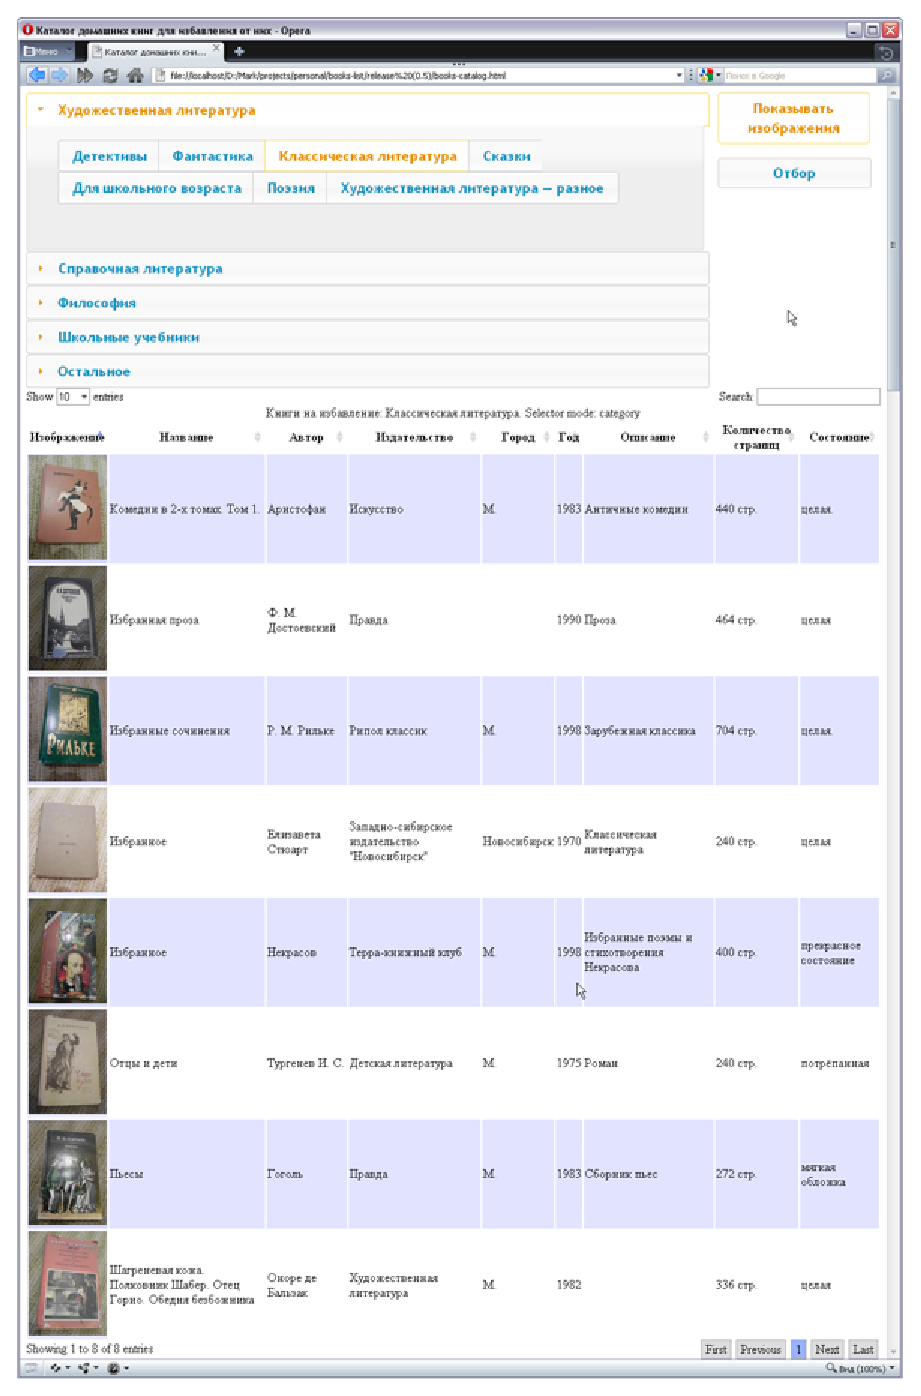
\includegraphics{book-catalog-screenshot.eps}
\end{center}
\caption{Каталог книг на экране}\label{book-catalog-screenshot}
\end{figure}

\chapter{Заключение}
По завершении работ поставленные цели были достигнуты и все задачи были решены полностью.

Присутствуют некоторые проблемы, выявленные при разработке (такие, как различия в поддержке XSLT в веб-браузерах) и некоторые проблемы, выявленные при тестировании (такие, как невозможность работы с каталогом через Сеть, несмотря на кажущуюся очевидность такой возможности). Однако, решение этих проблем не было связано с поставленными целями и задачами.

Данный каталог представляется удобным средством учёта книг в домашней библиотеке достаточно опытного пользователя персонального компьютера, способного редактировать текст и понимающего, что такое интерпретатор языка программирования и веб-браузер на уровне, достаточном для их использования.

Также появляется возможность переслать перечень имеющихся в наличии книг третьим лицам, без расчёта на наличие у них какого-либо специализированного программного обеспечения, кроме свежей версии веб-браузера.

\begin{thebibliography}{99}
\bibitem{Perl-website} The Perl Programming Language [В Интернете] // Веб-узел Perl.~--- 26 августа 2010.~--- http://www.perl.org/.
\bibitem{Perl-docs} Perl programming documentation --- perldoc.perl.org [В Интернете] // Веб-узел документации Perl.~--- 26 августа 2010.~--- http://perldoc.perl.org/.
\bibitem{ASPerl-website} Perl, Python and Tcl --- Dynamic Language Experts | ActiveState [В Интернете]  / ActiveState Software // Веб-узел ActiveState Perl.~--- 26 августа 2010.~--- http://www.activestate.com/
\bibitem{XSLT-o-reilly-book} XSLT, Second Edition, {\itshape Doug Tidwell}, 2008, O'Reilly Media, 992p, ISBN 978-0-596-52721-1.
\bibitem{Perl-o-reilly-book} Programming Perl, Third Edition, {\itshape Larry Wall, Tom Christiansen, Jon Orwant}, 2000, O'Reilly Media, 1104p, ISBN 978-0-596-00027-1.
\bibitem{regexp-book} Mastering Regular Expressions, Third Edition, {\itshape Jeffrey E.F.~Friedl}, 2006, O'Reilly Media, 544p, ISBN 978-0-596-52812-6.
\bibitem{Sarissa-website} Sarissa --- Sarissa Home Page [В Интернете] // Веб-узел Sarissa.~--- 26 августа 2010.~--- http://dev.abiss.gr/sarissa/.
\bibitem{jQuery-website} jQuery: The Write Less, Do More, JavaScript Library [В Интернете] // Веб-узел jQuery.~--- 26 августа 2010.~--- http://jquery.com/.
\bibitem{jQuery-DataTables} Plugins | jQuery Plugins [В Интернете] // Веб-архив плагинов к jQuery UI, плагин DataTables.~--- 26 августа 2010.~--- http://plugins.jquery.com/project/DataTables.
\bibitem{jQueryUI-website} jQuery UI --- Home [В Интернете] // Веб-узел jQuery UI.~--- 26 августа 2010.~--- http://jqueryui.com/.
\bibitem{jQueryUI-accordion} jQuery UI --- Accordion Demos and Documentation [В Интернете] // Веб-узел jQuery UI.~--- 26 августа 2010.~--- http://jqueryui.com/demos/accordion/.
\bibitem{jQueryUI-buttonset} jQuery UI --- Button Demos and Documentation [В Интернете] // Веб-узел jQuery UI.~--- 26 августа 2010.~--- http://jqueryui.com/demos/button/radio.html.
\bibitem{Mozilla-JS-XSLT-API} Using the Mozilla JavaScript interface to XSL Transformations [В Интернете] / Mozilla // Mozilla developer center.~--- 26 августа 2010.~--- https://developer.mozilla.org/en/\\using\_the\_mozilla\_javascript\_interface\_to\_xsl\_transformations.
\bibitem{XSLT-spec} XSL Transformations (XSLT) Version 1.0 [В Интернете] / W3C // Веб-узел World Wide Web Consortium.~--- 26 августа 2010.~--- http://www.w3.org/TR/xslt.
\bibitem{XPath-spec} XML Path Language (XPath) Version 1.0 [В Интернете] / W3C // Веб-узел World Wide Web Consortium.~--- 26 августа 2010.~--- http://www.w3.org/TR/xpath/.
\bibitem{XML-spec} Extensible Markup Language (XML) 1.0 (Fifth Edition) [В Интернете] / W3C // Веб-узел World Wide Web Consortium.~--- 26 августа 2010.~--- http://www.w3.org/TR/xml/.
\bibitem{XML-style-spec} Associating Style Sheets with XML documents Version 1.0 [В Интернете] / W3C // Веб-узел World Wide Web Consortium.~--- 26 августа 2010.~--- http://www.w3.org/TR/xml-stylesheet/.
\bibitem{XHTML-spec} XHTML 1.0 The Extensible HyperText Markup Language (Second Edition) [В Интернете] / W3C // Веб-узел World Wide Web Consortium.~--- 26 августа 2010.~--- http://www.w3.org/TR/xhtml1/.
\bibitem{HTML-spec} HTML 4.01 Specification [В Интернете] / W3C // Веб-узел World Wide Web Consortium.~--- 26 августа 2010.~--- http://www.w3.org/TR/html401/.
\bibitem{ECMAScript-spec} Standard ECMA-262 ECMAScript Language Specification 5th edition (December 2009) [В Интернете] / ECMA International // Веб-узел ECMA International.~--- 26 августа 2010.~--- http://www.ecma-international.org/publications/standards/Ecma-262.htm.
\bibitem{JSON-spec} Introducing JSON  [В Интернете] // Веб-узел JSON.~--- 26 августа 2010.~--- http://www.json.org/.
\bibitem{YAML-spec} YAML Ain’t Markup Language (YAML) Version 1.2  [В Интернете] // Веб-узел YAML.~--- 26 августа 2010.~--- http://yaml.org/spec/1.2/spec.html.

\end{thebibliography}
\end{document}
